\begin{frame}{Benutzerinteraktion}
	Bei der Benutzerinteraktion wurde der Großteil der Interaktionsmöglichkeiten durch Buttons und Pop-ups realisiert, um dem Nutzer eine möglichst simple Steuerung mit der Anwendung zu gewährleisten.
	
	\begin{center}
		\visible<2->{\stackunder[5pt]{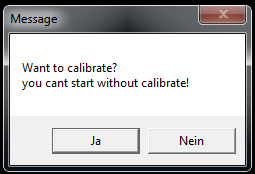
\includegraphics[height=2.1cm]{bilder/Calibrate-Popup.png}}{Kalibrierungs-Popup}}
		\visible<3->{\hspace{-0.0cm}\stackunder[5pt]{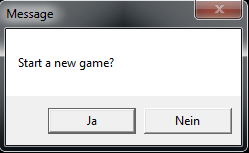
\includegraphics[height=2.1cm]{bilder/startGame-Popup.png}}{Starte Spiel-Popup}}
		\visible<4->{\hspace{-0.0cm}\stackunder[5pt]{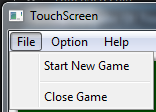
\includegraphics[height=2.1cm]{bilder/File-MenuBar.png}}{File-Menubar}}
		\visible<5->{\hspace{-0.0cm}\stackunder[5pt]{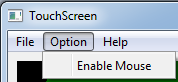
\includegraphics[height=2.1cm]{bilder/option-MenuBar.png}}{Option-Menubar}}
	\end{center}
\end{frame}

\begin{frame}{Benutzerinteraktion}
	Ein Teil dessen war allerdings auch das Anzeigen der Statistiken, worunter u.a. das Anzeigen des aktuellen Spielers oder der Kugelzuweisung fällt. Hierbei wurde die Variante gewählt, die Statistiken als Label auf dem Spielfeld anzeigen zu lassen.
	\begin{figure}[h]
		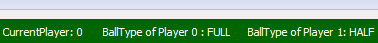
\includegraphics[width=\textwidth/1]{bilder/statisticLabel.png}
	\end{figure}
\end{frame}
